\section{Results}
\label{sec:res}

This section is structured as folows: First, Section~\ref{sec:seg4} demonstrates the level of segregation that can occur given our limited capability model with 4 neurons; Section~\ref{sec:seg6} demonstrates the behavior of a 6 neuron model; finally, Section~\ref{sec:fitness} discusses the performance our fitness search model. 


\subsection{Segregation with 4-neuron capability model}
\label{sec:seg4}

Our key contribution is to determine whether we can observe segregation with our given capability model. 
To determine this, we the previously described novelty search algorithm for 100 generations.
During each generation, we tested \emph{all permutations} of the 4 neuron weights with a step size of 0.1, which ensures that each step discover the true `most novel' new population.

At the end of this process, the population which demonstrated the highest segregation score had the weights $[0.61, 0.59, 0.01, 0.3]$. 
This can be interpreted as follows: when bot \emph{A} sees bot \emph{B} of the same type, it uses the first weights 0.61 and 0.59 to control its wheels.
This results in bot \emph{A} quickly moving generally straight (with a slight turn) towards the bot \emph{B}. 
When bot \emph{A} sees eithe nothing \emph{or} a bot of any other type, then the bot will use the second set of weights, 0.1, 0.3, to control its left and right wheels respectivly. 
This results in the bot mostly spinning in place until it sees a bot of the same type. 

This behavior can be seen in Figure~\ref{fig:init_pos_1} which depicts the positions of the bots over the course of the simulation. 
The colored depict the location of the bots at the start of the simulation and the light colored paths depict the locations of where the bots will travel. 
As seen here, the bots are evenly dispered at the start of the simulation, and thus not segregated.
The circling behavior can be seen at locations $X= 0$, $Y= -1.5$. 
The paths of the bots are drawn with low opacity, so the dark circle here demonstrates that a bot spent a great deal of time circling this location. 


\begin{figure}
    \centering
    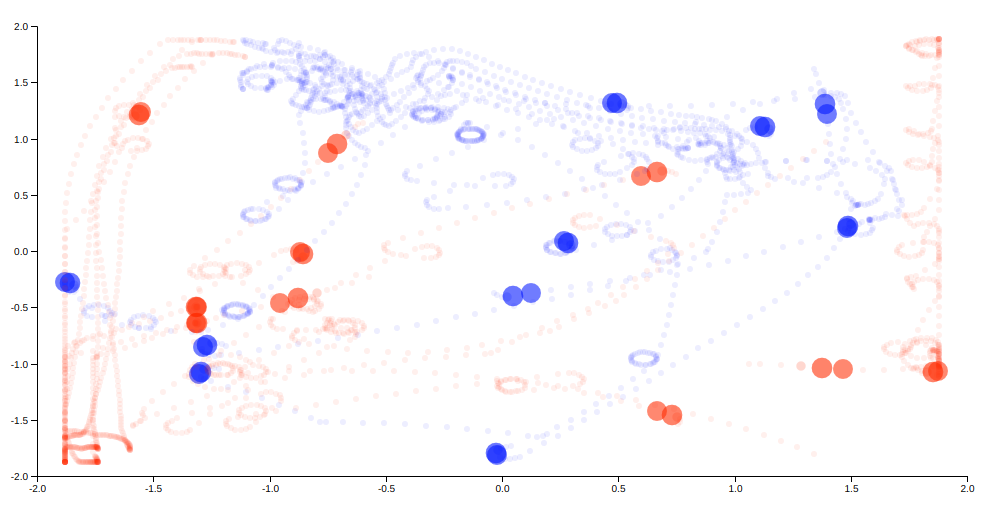
\includegraphics[width=\linewidth]{imgs/init_place_1.png}
    \caption{Positions of bots at the start of the simulation}
    \label{fig:init_pos_1}
\end{figure}

Figure~\ref{fig:final_seg_1} depicts our calculated segregation score for this population during each iteration. 
The highest segregation can be seen around step 2,400. 
The three values used to calulate this metric over the same time period are shown in Figure~\ref{fig:final_dev_1}. 
The line represent the standard deviation of the distances from the bots to the metroid of the cluster for each swarm with red line corresponding to the red group, the blue corresponding to the blue group, and the gray line corresponding to the total standard deviation of distances to the center of all bots. 
The dark colored dot depcits the current time in our animation~\footnote{We use a an interactive animation to depict these results. github:

\url{http://tiny.cc/e4hv5y}}.
Figure~\ref{fig:final_pos_1} demonstates the location of the bots during this point of highest segregation. 
As expected, when the bots look visually segregated, the intra-group standard deviations of their positions are low and the inter-group deviations are high (Figure~\ref{fig:final_dev_1}), and this corresponds to a high numeric value of segregation (Figure~\ref{fig:final_seg_1}). 

\begin{figure}
    \centering
    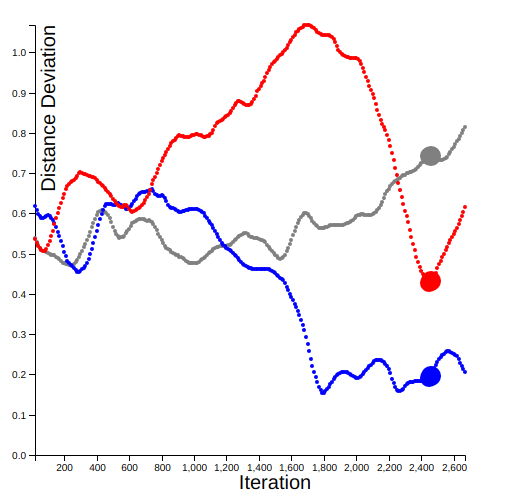
\includegraphics[width=5.5cm]{imgs/final_dev_1.png}
    \caption{Standard deviations of inter and intra-group distances for each population}
    \label{fig:final_dev_1}
\end{figure}

\begin{figure}
    \centering
    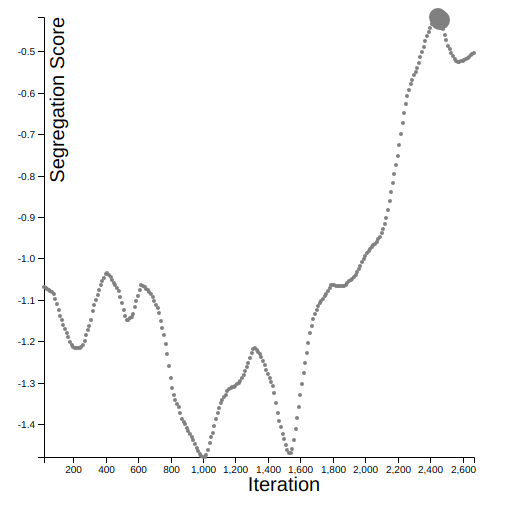
\includegraphics[width=5.5cm]{imgs/final_seg_1.png}
    \caption{Segregation score of the population at each time step}
    \label{fig:final_seg_1}
\end{figure}

\begin{figure}
    \centering
    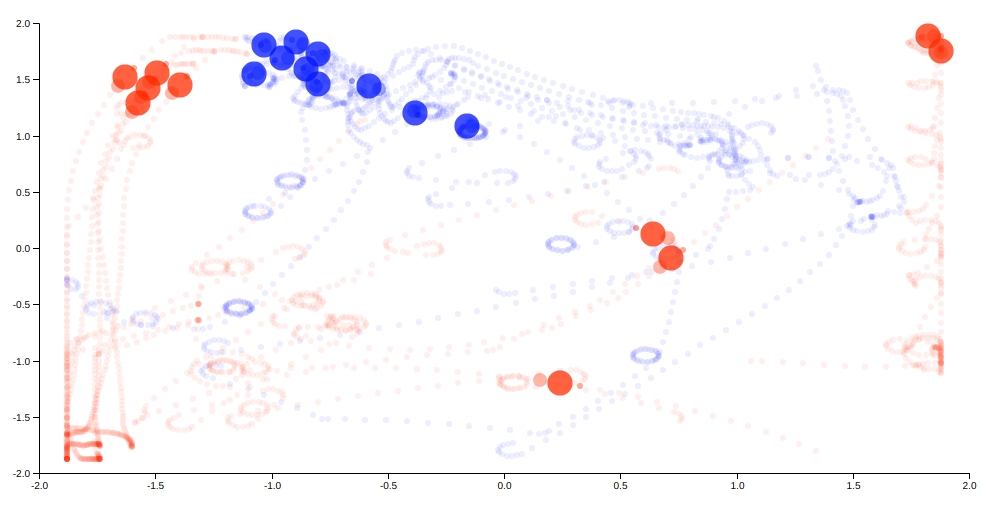
\includegraphics[width=\linewidth]{imgs/final_place_1.png}
    \caption{Positions of bots at the location of the highest clustering}
    \label{fig:final_pos_1}
\end{figure}

\subsection{Dispersion test}
\label{sec:dispersion}

To validate our segregation metrics, we hand-coded a population that would create high dispersal. 
We did this by setting the weights to $[.3, .3, .3, .3, .3, .3]$.
Using these weights, the bots would \emph{always} move straight forward at a slow speed.
The results for this format can be seen in Figures~\ref{fig:final_dev_d}, \ref{fig:final_seg_d}, and \ref{fig:final_pos_d} depict the results in a similar format to the above images. 
As seen here, the bots move straight until they reach the edge of the map, at which point they continue to move straight but are largely stationary. 
Thus, the standard deviation in the positions (Figure\ref{fig:final_dev_d}) remains fairly uniform across all of the clusters - there is no extra clustering between groups of the same type. 
The segregation score depicted in \ref{fig:final_seg_d} also remains very low, reflecting the low preference for segregation exhibited by this population.
This serves as a sort of validation that our segregation metric is able to descriminate against poorly segregated populations, and that our capability can still exhibit some forms of segregations.

\begin{figure}
    \centering
    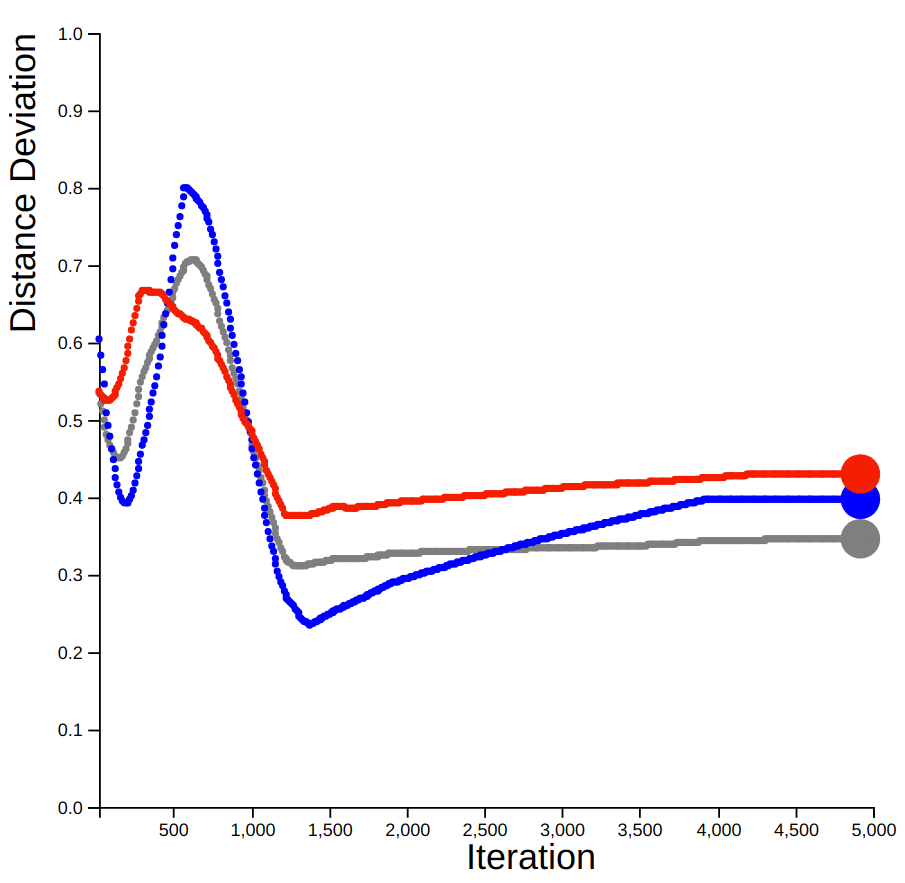
\includegraphics[width=5.5cm]{imgs/final_dev_d.png}
    \caption{Standard deviations of inter and intra-group distances for each cluster of high-dispersal population}
    \label{fig:final_dev_d}
\end{figure}

\begin{figure}
    \centering
    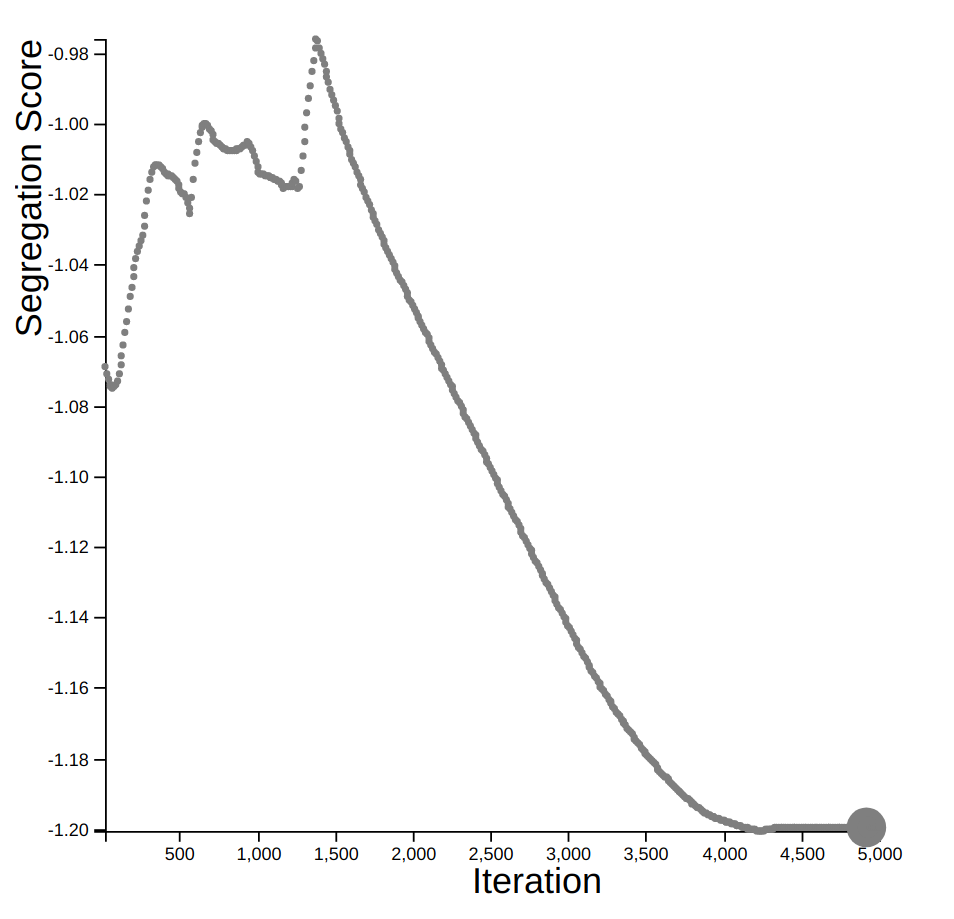
\includegraphics[width=5.5cm]{imgs/final_seg_d.png}
    \caption{Segregation score of the population at each time step for high-dispersal population}
    \label{fig:final_seg_d}
\end{figure}

\begin{figure}
    \centering
    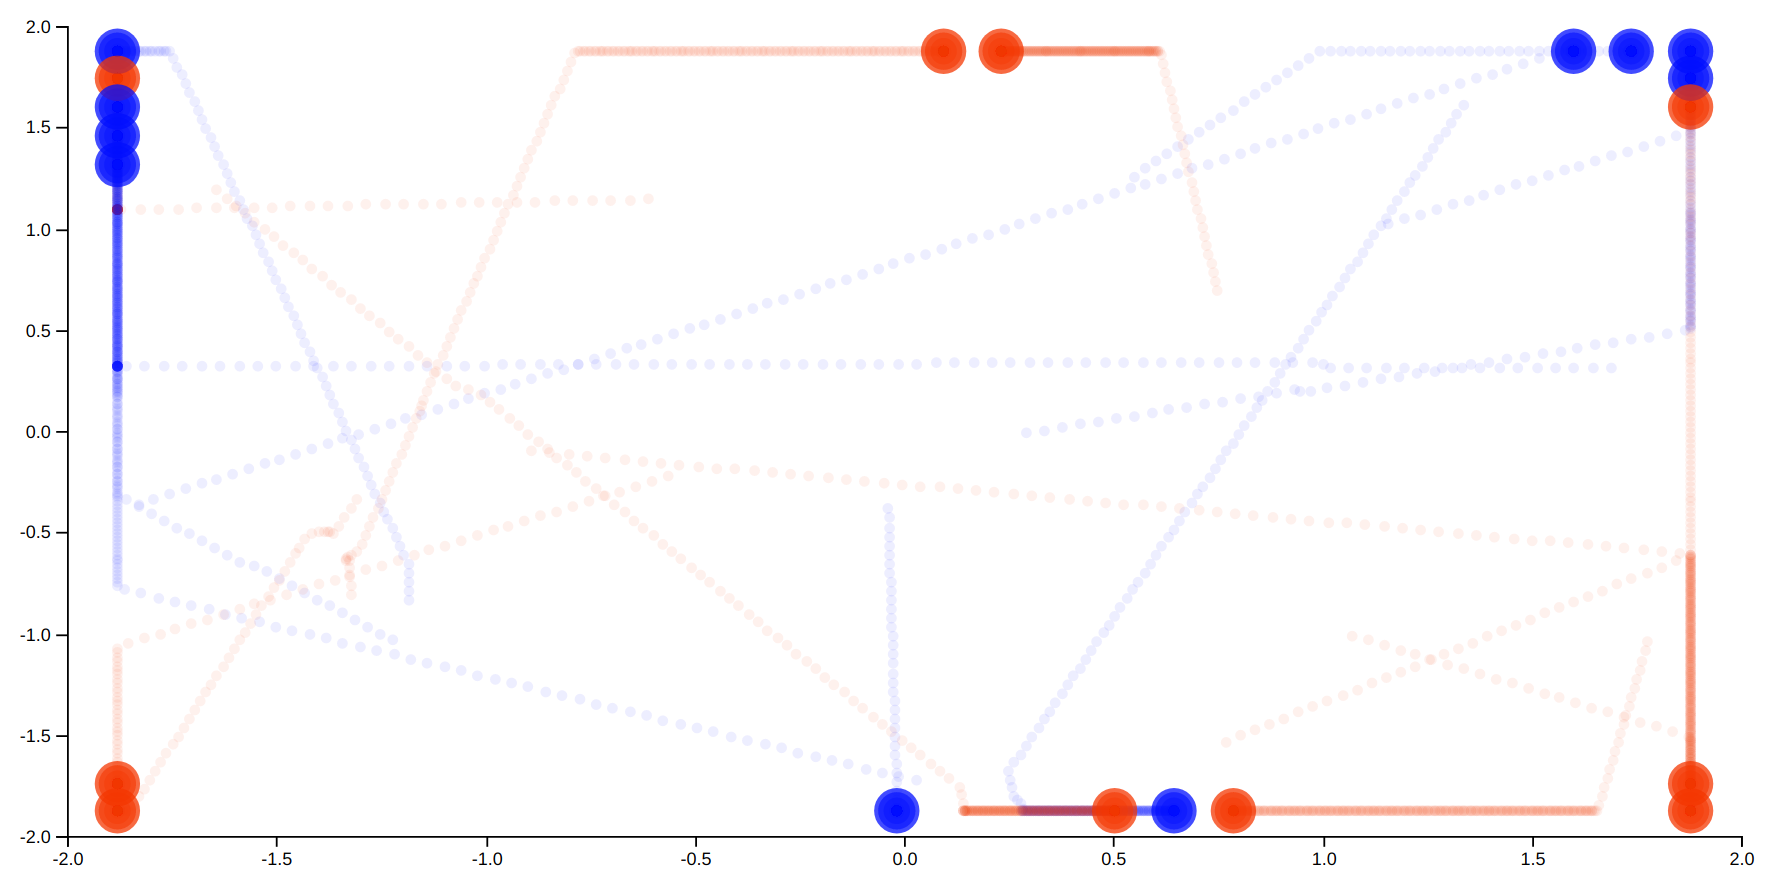
\includegraphics[width=\linewidth]{imgs/final_place_d.png}
    \caption{Positions at the end of the simulation for high dispersal population}
    \label{fig:final_pos_d}
\end{figure}



\subsection{Segregation with 6-neuron capability model}
\label{sec:seg6}



\subsection{Fitness search performance}
\label{sec:fitness}

After running the experiments above, we determined that a novelty search is not the most efficient technique for our problem. 
Where a novelty search worked well for Brown et. al. who were trying to categorize \emph{all} possible behaviors exhibited by the capability model, we were only interested in determining one behavior - segregation.
And, as we already determined a valid measure of segregation for our model, we were able to refit our evolutionary search using a fitness function that favors segregation instead of novelty. 
Thus, at each generation of the evolutionary search, we sort the new populations by their segregation scores. 
Then, rather than permuting the most novel population from these new populations, we instead permute the most segregated population.

After 100 generations, the most segregated population has the weights $[0.56, 0.46, 0.21, 0.31]$, which is slightly different from the most segregated population discovered by the original novelty search. 
The behavior of this population is summarized in the above format in Figures~\ref{fig:final_dev_2}, \ref{fig:final_seg_2}, and \ref{fig:final_pos_2}. 
As seen in Figure~\ref{fig:final_seg_2}, the segregation for this population is high, peaking at around $-0.6$, which is slightly higher than the highest segregation exhibited by the best novely search result. 

We also plot the highest segregation of each generation in Figure~\ref{fig:gen_fitness}. 
In general, each generation is able to find a better segregating population than the previous, and this seems to have diminishing returns as the simulation goes on\footnote{Note that this function is roughly bounded between zero and one, so it must have asymptotic functions over time}. 
Also, as seen in the previous sections, the segregation scores for the populations is not very stable, and it can fluctuate greatly between each time step for a single population. 
To generate this figure, we took the last time step's segregation score, which may not have been the highest segregation score exhibited over the course of that population's runtime. 

\begin{figure}
    \centering
    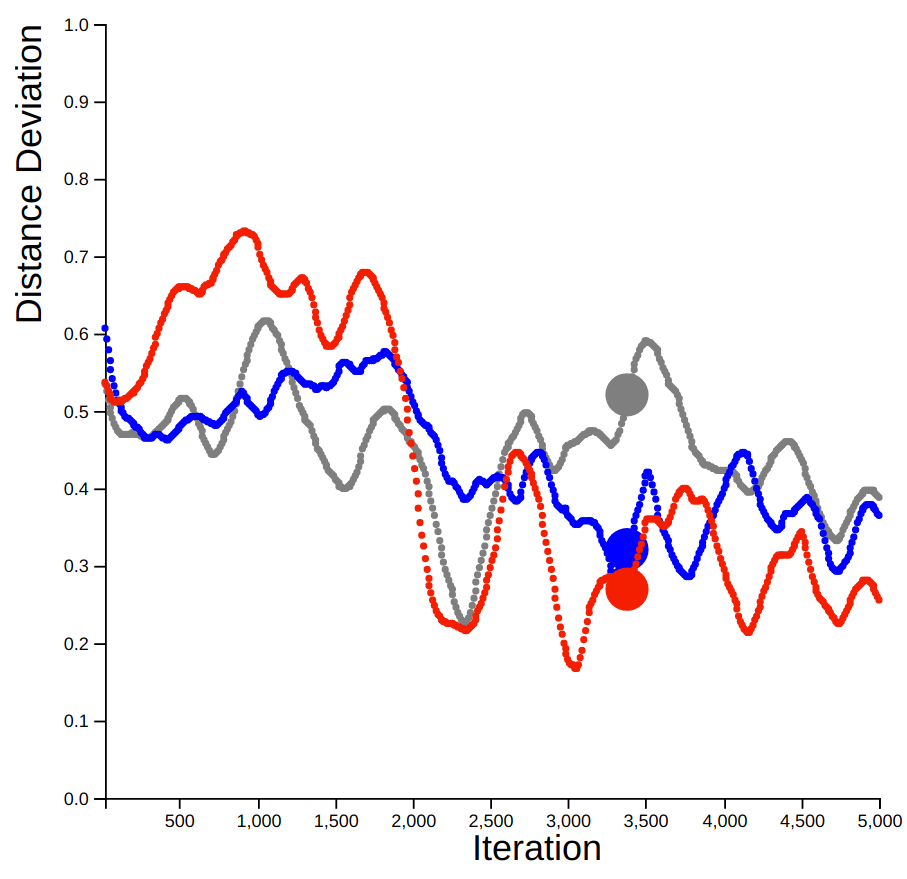
\includegraphics[width=5.5cm]{imgs/final_dev_2.png}
    \caption{Standard deviations of inter and intra-group distances for each robot in fitness search population}
    \label{fig:final_dev_2}
\end{figure}

\begin{figure}
    \centering
    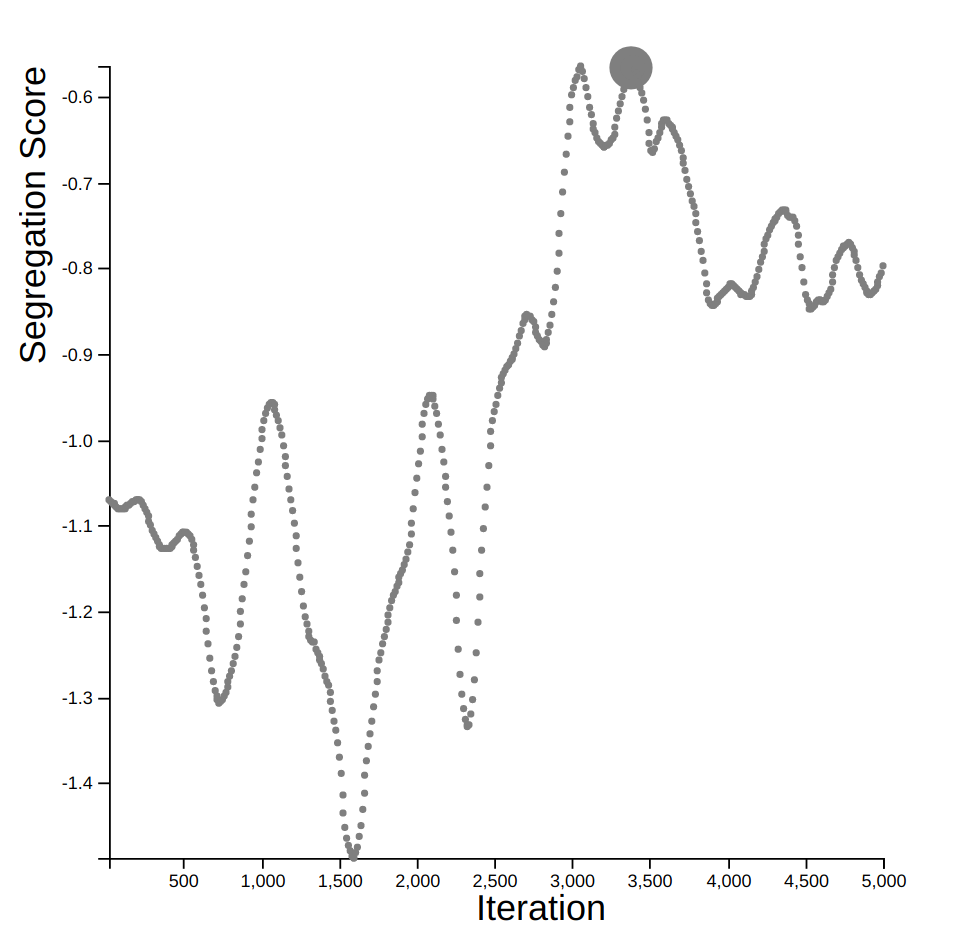
\includegraphics[width=5.5cm]{imgs/final_seg_2.png}
    \caption{Segregation score of the population at each time step in fitness search population}
    \label{fig:final_seg_2}
\end{figure}

\begin{figure}
    \centering
    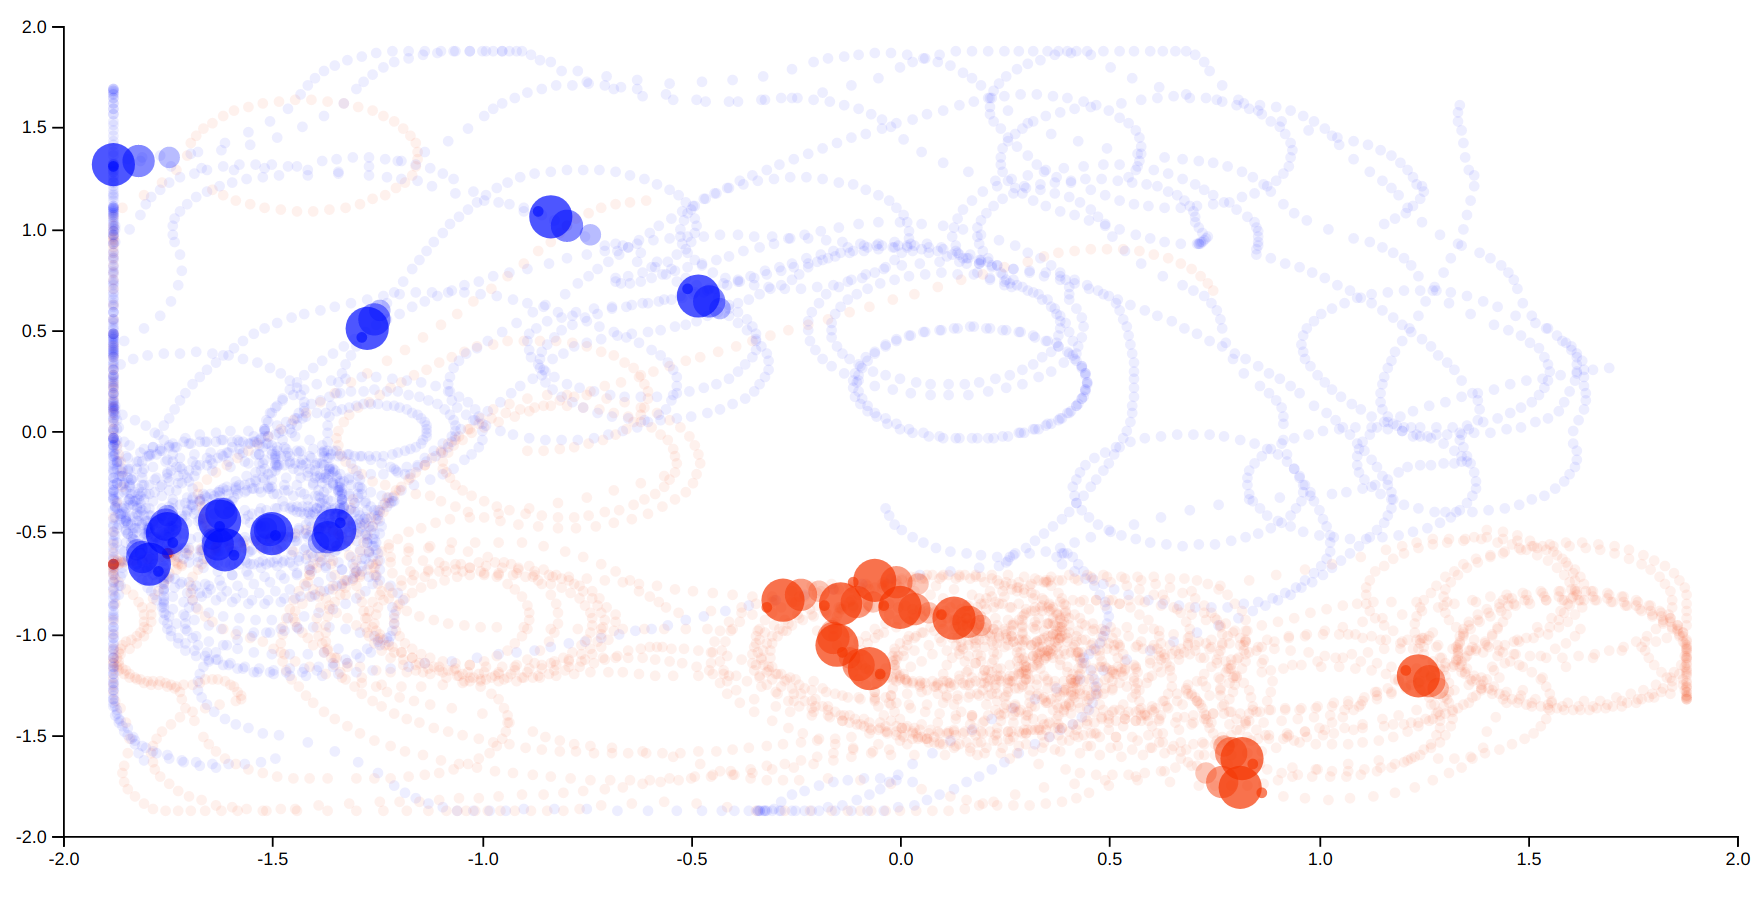
\includegraphics[width=\linewidth]{imgs/final_place_2.png}
    \caption{Positions of bots at the location of the highest clustering in fitness search population}
    \label{fig:final_pos_2}
\end{figure}

\begin{figure}
    \centering
    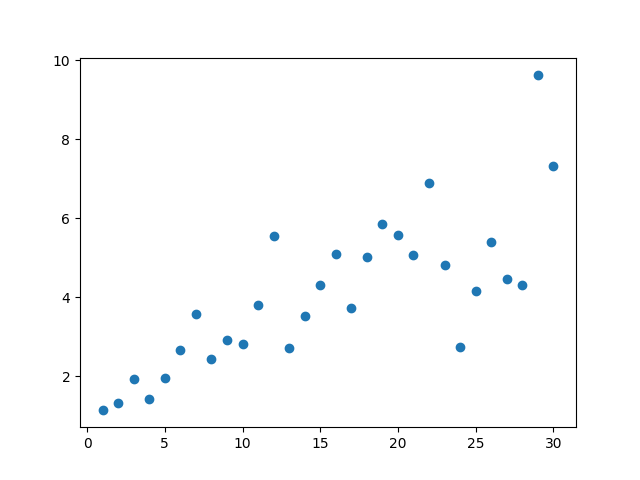
\includegraphics[width=\linewidth]{imgs/fitness_search.png}
    \caption{Maximum fitness observed in each generation}
    \label{fig:final_pos_2}
\end{figure}
